\begin{frame}[fragile]

  {\Huge Kokkos Kernels: Library Based Approach for Performance Portable Sparse/Dense linear algebra and Graph Kernels}

  \vspace{20pt}

  \textbf{Presented by:}

  Siva Rajamanickam, S. Acer, L. Berger-Vergiat, V. Dang, N. Ellingwood, E.
  Harvey, B. Kelley, K. Kim, C.R. Trott, J. Wilke

  \vspace{-20pt}

\end{frame}

%==========================================================================

\begin{frame}[fragile]{Module 8: Kernels Math Libraries}

\textbf{Kokkos Ecosystem for Performance Portability}

  \begin{columns}[t,onlytextwidth]
    \column{.75\textwidth}
    \begin{center}
      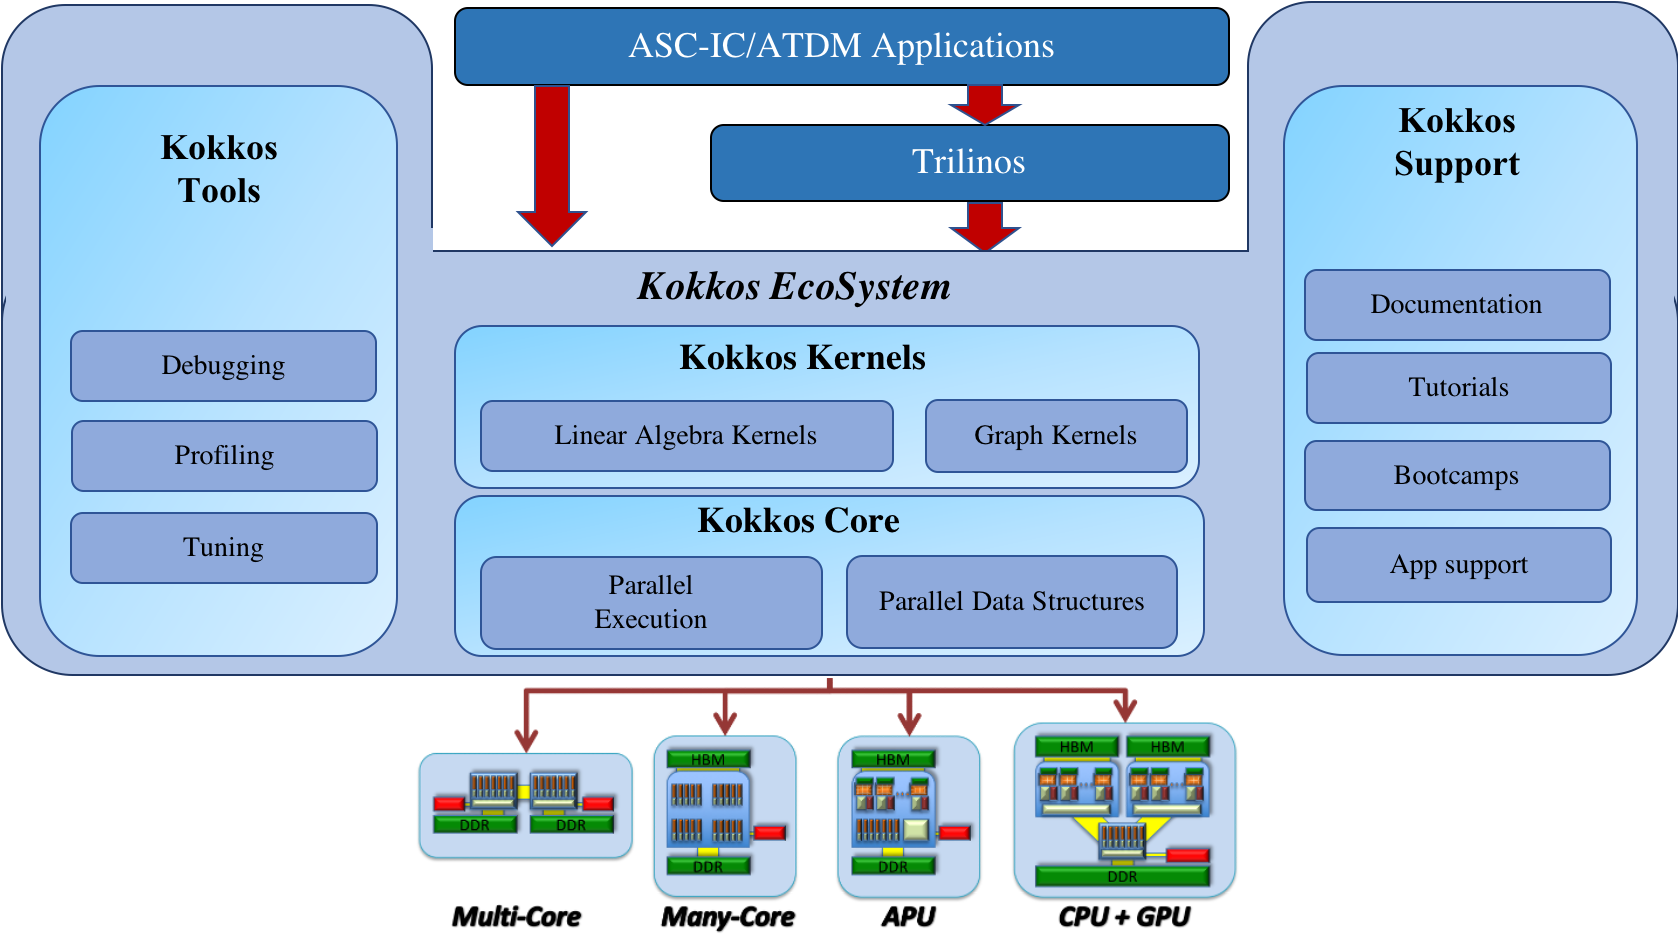
\includegraphics[width=0.95\textwidth]{figures/kernels-ecosystem}
    \end{center}

%    \begin{lstlisting}[frame=single, backgroundcolor=\color{blue!10}, basicstyle=\tiny, breaklines=true, boxpos=c]
%      Kokkos Ecosystem addresses complexity of supporting numerous many/multi-core architectures that are central to DOE HPC enterprise
%    \end{lstlisting}

    \column{.25\textwidth}
    \scriptsize{\textbf{Kokkos Core}: parallel patterns and data structures; supports several execution and memory spaces}
\\
    \scriptsize{\textbf{Kokkos Kernels}: performance portable BLAS; sparse, dense and graph algorithms}
\\
    \scriptsize{\textbf{Kokkos Tools}: debugging and profiling support}

%    \begin{lstlisting}[frame=single, backgroundcolor=\color{gray!10}, basicstyle=\tiny, breaklines=true]
%      Write - once using Kokkos for portable performance on different architectures
%    \end{lstlisting}

  \end{columns}

  \begin{lstlisting}[frame=single, backgroundcolor=\color{blue!10}, basicstyle=\tiny, breaklines=true, boxpos=c]
    Kokkos Ecosystem addresses complexity of supporting numerous many/multi-core architectures that are central to DOE HPC enterprise
  \end{lstlisting}

\end{frame}

%==========================================================================

\begin{frame}[fragile]{Focus of Kokkos Kernels}

Deliver \textbf{portable} sparse/dense linear algebra and graph kernels
\begin{itemize}
  \item These are the kernels that are in 80\% of time for most applications
  \item Key problems: Kernels might need different algorithms/implementations to get the best performance
  \item Ninja programming needs in addition to Kokkos
  \item Users of the kernels do not need to be ninja programmers
  \item \textbf{Focus on performance of the kernels on all the platforms of interest to DOE}
\end{itemize}

\begin{textblock*}{1.0\textwidth}(.1\textwidth,0.80\textheight)
  \begin{lstlisting}[frame=single, backgroundcolor=\color{blue!10}, basicstyle=\tiny, breaklines=true, boxpos=c]
    Kokkos Kernels delivers portable, high-performance kernels in a robust software ecosystem to support CSE applications
  \end{lstlisting}
\end{textblock*}

\end{frame}

\begin{frame}[fragile]{Focus of Kokkos Kernels}

Deliver \textbf{robust software ecosystem} for other software technology projects and applications
\begin{itemize}
  \item Production software capabilities that give high performance, portable and turn-key
  \item Tested on number of configurations nightly  (architectures, compilers, debug/optimized, programming model backend, complex/real, ordinal types...)
  \item Larger release/integration testing with Trilinos and applications
  \item Kokkos Support, github issues, tutorials, hackathons, user group meetings, slack
\end{itemize}

\begin{textblock*}{1.0\textwidth}(.1\textwidth,0.80\textheight)
  \begin{lstlisting}[frame=single, backgroundcolor=\color{blue!10}, basicstyle=\tiny, breaklines=true, boxpos=c]
    Kokkos Kernels delivers portable, high-performance kernels in a robust software ecosystem to support CSE applications
  \end{lstlisting}
\end{textblock*}

\end{frame}


\begin{frame}[fragile]{Focus of Kokkos Kernels}

Serve as \textbf{reference implementation} of key kernel needs of applications
\begin{itemize}
  \item Actively work with vendors to develop high performance implementation in their libraries
  \item Provide interface to vendor implementations where they are better
  \item Actively publish the algorithms so the community develops even better variations
\end{itemize}

\begin{textblock*}{1.0\textwidth}(.1\textwidth,0.80\textheight)
  \begin{lstlisting}[frame=single, backgroundcolor=\color{blue!10}, basicstyle=\tiny, breaklines=true, boxpos=c]
    Kokkos Kernels delivers portable, high-performance kernels in a robust software ecosystem to support CSE applications
  \end{lstlisting}
\end{textblock*}

\end{frame}

\begin{frame}[fragile]{Focus of Kokkos Kernels}

Actively partner with Applications to identify new opportunities for performance
\begin{itemize}
  \item Actively publish the algorithms so the community develops even better variations
  \item \textbf{Team-level dense, sparse linear algebra}
  \item \textbf{Team-level data structures (hashmap) and utilities (sorting) for better performance}
  \item \textbf{Fused Kernels}
  \item \textbf{Symbolic and Numeric separation in interface design}
\end{itemize}

\begin{textblock*}{1.0\textwidth}(.1\textwidth,0.80\textheight)
  \begin{lstlisting}[frame=single, backgroundcolor=\color{blue!10}, basicstyle=\tiny, breaklines=true, boxpos=c]
    Kokkos Kernels delivers portable, high-performance kernels in a robust software ecosystem to support CSE applications
  \end{lstlisting}
\end{textblock*}

\end{frame}


\begin{frame}[fragile]{Collaborations with Vendors}

\textbf{NVIDIA}
\begin{itemize}
  \item Summit on Summit meetings
  \item Biweekly work stream meetings to guide NVIDIA's math libraries plans
  \item Kernel requirements prioritized by application needs and milestones
  \item Long history of interaction as part of COE
  \item SpGEMM, GEMM, Solvers are all improved
\end{itemize}

\textbf{ARM}
\begin{itemize}
  \item Working with the math libraries team both on algorithms
  \item SpGEMM, SpMV, Batched linear algebra in ARM PL
\end{itemize}

%\begin{textblock*}{1.0\textwidth}(.1\textwidth,0.83\textheight)
%  \begin{lstlisting}[frame=single, backgroundcolor=\color{blue!10}, basicstyle=\tiny, breaklines=true, boxpos=c]
%    Kokkos Kernels team working with hardware vendors to support application 
%    needs on current and exascale platforms
%  \end{lstlisting}
%\end{textblock*}

\end{frame}

\begin{frame}[fragile]{Collaborations with Vendors}

\textbf{AMD}
\begin{itemize}
  \item Just started the interactions on sparse, dense, batched linear algebra kernels, and sparse solvers
  \item Kokkos backend under-development
  \item Kokkos Kernels will be the performance test case
\end{itemize}

\textbf{Intel}
\begin{itemize}
  \item Compact API on KNL
  \item Kokkos backend under development
  \item Kokkos Kernels will be the performance test case
\end{itemize}

\begin{textblock*}{1.0\textwidth}(.1\textwidth,0.83\textheight)
  \begin{lstlisting}[frame=single, backgroundcolor=\color{blue!10}, basicstyle=\tiny, breaklines=true, boxpos=c]
    Kokkos Kernels team working with hardware vendors to support application 
    needs on current and exascale platforms
  \end{lstlisting}
\end{textblock*}

\end{frame}


\begin{frame}[fragile]{Collaborations with ECP Applications}

\textbf{SPARC}:  state-of-the-art hypersonic unsteady hybrid structured/unstructured finite volume CFD code
\begin{itemize}
  \item \textbf{High performance line solvers; batched BLAS on CPUs and GPUs}
  \item \textbf{Performance-portable programming models}
\end{itemize}

\textbf{EMPIRE}: next-gen unstructured-mesh FEM PIC/multifluid plasma simulation code
\begin{itemize}
  \item Scalable solvers for electrostatic and electromagnetic systems for Trinity and Sierra architectures
  \item \textbf{Thread-scalable, performance-portable, on-node linear algebra kernels to support multigrid methods}
  \item \textbf{Performance-portable programming models}
  \item Non-linear solvers, discretization, and automatic differentiation approaches
\end{itemize}

%\begin{textblock*}{1.0\textwidth}(.1\textwidth,0.83\textheight)
%  \begin{lstlisting}[frame=single, backgroundcolor=\color{blue!10}, basicstyle=\tiny, breaklines=true, boxpos=c]
%    Kokkos Kernels integrated into several applications in an agile manner at 
%    all stages from requirements solicitation, designing kernels and integration
%  \end{lstlisting}
%\end{textblock*}

\end{frame}

\begin{frame}[fragile]{Collaborations with ECP Applications}

\textbf{Exawind}: next-gen wind simulation code
\begin{itemize}
  \item \textbf{Scalable solvers for Trinity and Sierra architectures}
  \item \textbf{Thread-scalable, performance-portable, on-node linear algebra kernels to support multigrid methods}
  \item \textbf{Performance-portable programming models}
\end{itemize}

\textbf{QMCPACK}: Electronic structure code with Quantum Monte Carlo Algorithms
\begin{itemize}
  \item Team level BLAS and LAPACK within the Kokkos ecssytem
\end{itemize}

\begin{textblock*}{1.0\textwidth}(.1\textwidth,0.83\textheight)
  \begin{lstlisting}[frame=single, backgroundcolor=\color{blue!10}, basicstyle=\tiny, breaklines=true, boxpos=c]
    Kokkos Kernels integrated into several applications in an agile manner at 
    all stages from requirements solicitation, designing kernels and integration
  \end{lstlisting}
\end{textblock*}

\end{frame}


